
\documentclass[letterpaper,hide notes,xcolor={table,svgnames},pdftex,10pt]{beamer}
\def\showexamples{t}

\usecolortheme{crane}
\setbeamertemplate{navigation symbols}{}

\usetheme{MyPittsburgh}
\usepackage{hyperref}
\usepackage{graphicx,xspace}
\usepackage[normalem]{ulem}
\usepackage{multicol}
\usepackage{amsmath,amssymb,amsthm,graphicx,xspace}
\newcommand\SF[1]{$\bigstar$\footnote{SF: #1}}

\usepackage[sfdefault,lf]{carlito}
\usepackage[T1]{fontenc}
\usepackage[scaled]{beramono}
\usepackage{tikzpagenodes}
\newcommand{\Rplus}{\protect\hspace{-.1em}\protect\raisebox{.35ex}{\small{\small\textbf{+}}}}
\newcommand{\Cpp}{\mbox{C\Rplus\Rplus}\xspace}

\newcounter{tmpnumSlide}
\newcounter{tmpnumNote}

\newcommand\mnote[1]{%
	\addtocounter{tmpnumSlide}{1}
	\ifdefined\showcues {~\tiny\fbox{\arabic{tmpnumSlide}}}\fi
	\note{\setlength{\parskip}{1ex}\addtocounter{tmpnumNote}{1}\textbf{\Large \arabic{tmpnumNote}:} {#1\par}}}

\newcommand\mmnote[1]{\note{\setlength{\parskip}{1ex}#1\par}}


\newcommand\mquestion[2]{{~\color{red}\fbox{?}}\note{\setlength{\parskip}{1ex}\par{\Large \textbf{?}} #1} \note{\setlength{\parskip}{1ex}\par{\Large \textbf{A}} #2\par}\ifdefined \presentationonly \pause \fi}

\newcommand\blackboard[1]{%
	\ifdefined   \showblackboard
		{#1}
	\else {\begin{center} \fbox{\colorbox{blue!30}{%
						\begin{minipage}{.95\linewidth}%
							\hspace{\stretch{1}} Some space intentionally left blank; done at the blackboard.%
						\end{minipage}}}\end{center}}%
	\fi%
}

\usepackage{listings}
\lstset{%
	keywordstyle=\bfseries,
	aboveskip=15pt,
	belowskip=15pt,
	captionpos=b,
	identifierstyle=\ttfamily,
	frame=lines,
	numbers=left, basicstyle=\scriptsize, numberstyle=\tiny, stepnumber=0, numbersep=2pt}

\usepackage{siunitx}
\newcommand\sius[1]{\num[group-separator = {,}]{#1}\si{\micro\second}}
\newcommand\sims[1]{\num[group-separator = {,}]{#1}\si{\milli\second}}
\newcommand\sins[1]{\num[group-separator = {,}]{#1}\si{\nano\second}}
\sisetup{group-separator = {,}, group-digits = true}

%% -------------------- tikz --------------------
\usepackage{tikz}
\usetikzlibrary{positioning}
\usetikzlibrary{arrows,backgrounds,automata,decorations.shapes,decorations.pathmorphing,decorations.markings,decorations.text}

\tikzstyle{place}=[circle,draw=blue!50,fill=blue!20,thick, inner sep=0pt,minimum size=6mm]
\tikzstyle{transition}=[rectangle,draw=black!50,fill=black!20,thick, inner sep=0pt,minimum size=4mm]

\tikzstyle{block}=[rectangle,draw=black, thick, inner sep=5pt]
\tikzstyle{bullet}=[circle,draw=black, fill=black, thin, inner sep=2pt]

\tikzstyle{pre}=[<-,shorten <=1pt,>=stealth',semithick]
\tikzstyle{post}=[->,shorten >=1pt,>=stealth',semithick]
\tikzstyle{bi}=[<->,shorten >=1pt,shorten <=1pt, >=stealth',semithick]

\tikzstyle{mut}=[-,>=stealth',semithick]

\tikzstyle{treereset}=[dashed,->, shorten >=1pt,>=stealth',thin]

\usepackage{ifmtarg}
\usepackage{xifthen}
\makeatletter
% new counter to now which frame it is within the sequence
\newcounter{multiframecounter}
% initialize buffer for previously used frame title
\gdef\lastframetitle{\textit{undefined}}
% new environment for a multi-frame
\newenvironment{multiframe}[1][]{%
	\ifthenelse{\isempty{#1}}{%
		% if no frame title was set via optional parameter,
		% only increase sequence counter by 1
		\addtocounter{multiframecounter}{1}%
	}{%
		% new frame title has been provided, thus
		% reset sequence counter to 1 and buffer frame title for later use
		\setcounter{multiframecounter}{1}%
		\gdef\lastframetitle{#1}%
	}%
	% start conventional frame environment and
	% automatically set frame title followed by sequence counter
	\begin{frame}%
		\frametitle{\lastframetitle~{\normalfont(\arabic{multiframecounter})}}%
		}{%
	\end{frame}%
}
\makeatother

\makeatletter
\newdimen\tu@tmpa%
\newdimen\ydiffl%
\newdimen\xdiffl%
\newcommand\ydiff[2]{%
	\coordinate (tmpnamea) at (#1);%
	\coordinate (tmpnameb) at (#2);%
	\pgfextracty{\tu@tmpa}{\pgfpointanchor{tmpnamea}{center}}%
	\pgfextracty{\ydiffl}{\pgfpointanchor{tmpnameb}{center}}%
	\advance\ydiffl by -\tu@tmpa%
}
\newcommand\xdiff[2]{%
	\coordinate (tmpnamea) at (#1);%
	\coordinate (tmpnameb) at (#2);%
	\pgfextractx{\tu@tmpa}{\pgfpointanchor{tmpnamea}{center}}%
	\pgfextractx{\xdiffl}{\pgfpointanchor{tmpnameb}{center}}%
	\advance\xdiffl by -\tu@tmpa%
}
\makeatother
\newcommand{\copyrightbox}[3][r]{%
	\begin{tikzpicture}%
		\node[inner sep=0pt,minimum size=2em](ciimage){#2};
		\usefont{OT1}{phv}{n}{n}\fontsize{4}{4}\selectfont
		\ydiff{ciimage.south}{ciimage.north}
		\xdiff{ciimage.west}{ciimage.east}
		\ifthenelse{\equal{#1}{r}}{%
			\node[inner sep=0pt,right=1ex of ciimage.south east,anchor=north west,rotate=90]%
			{\raggedleft\color{black!50}\parbox{\the\ydiffl}{\raggedright{}#3}};%
		}{%
			\ifthenelse{\equal{#1}{l}}{%
				\node[inner sep=0pt,right=1ex of ciimage.south west,anchor=south west,rotate=90]%
				{\raggedleft\color{black!50}\parbox{\the\ydiffl}{\raggedright{}#3}};%
			}{%
				\node[inner sep=0pt,below=1ex of ciimage.south west,anchor=north west]%
				{\raggedleft\color{black!50}\parbox{\the\xdiffl}{\raggedright{}#3}};%
			}
		}
	\end{tikzpicture}
}


%% --------------------

%\usepackage[excludeor]{everyhook}
%\PushPreHook{par}{\setbox0=\lastbox\llap{MUH}}\box0}

%\vspace*{\stretch{1}

%\setbox0=\lastbox \llap{\textbullet\enskip}\box0}

\setlength{\parskip}{\fill}

\newcommand\noskips{\setlength{\parskip}{1ex}}
\newcommand\doskips{\setlength{\parskip}{\fill}}

\newcommand\xx{\par\vspace*{\stretch{1}}\par}
\newcommand\xxs{\par\vspace*{2ex}\par}
\newcommand\tuple[1]{\langle #1 \rangle}
\newcommand\code[1]{{\sf \footnotesize #1}}
\newcommand\ex[1]{\uline{Example:} \ifdefined \presentationonly \pause \fi
	\ifdefined\showexamples#1\xspace\else{\uline{\hspace*{2cm}}}\fi}

\newcommand\ceil[1]{\lceil #1 \rceil}


\AtBeginSection[]
{
	\begin{frame}
		\frametitle{Outline}
		\tableofcontents[currentsection]
	\end{frame}
}



\pgfdeclarelayer{edgelayer}
\pgfdeclarelayer{nodelayer}
\pgfsetlayers{edgelayer,nodelayer,main}

\tikzstyle{none}=[inner sep=0pt]
\tikzstyle{rn}=[circle,fill=Red,draw=Black,line width=0.8 pt]
\tikzstyle{gn}=[circle,fill=Lime,draw=Black,line width=0.8 pt]
\tikzstyle{yn}=[circle,fill=Yellow,draw=Black,line width=0.8 pt]
\tikzstyle{empty}=[circle,fill=White,draw=Black]
\tikzstyle{bw} = [rectangle, draw, fill=blue!20,
text width=4em, text centered, rounded corners, minimum height=2em]

\newcommand{\CcNote}[1]{% longname
	This work is licensed under the \textit{Creative Commons #1 3.0 License}.%
}
\newcommand{\CcImageBy}[1]{%
	\includegraphics[scale=#1]{creative_commons/cc_by_30.pdf}%
}
\newcommand{\CcImageSa}[1]{%
	\includegraphics[scale=#1]{creative_commons/cc_sa_30.pdf}%
}
\newcommand{\CcImageNc}[1]{%
	\includegraphics[scale=#1]{creative_commons/cc_nc_30.pdf}%
}
\newcommand{\CcGroupBySa}[2]{% zoom, gap
	\CcImageBy{#1}\hspace*{#2}\CcImageNc{#1}\hspace*{#2}\CcImageSa{#1}%
}
\newcommand{\CcLongnameByNcSa}{Attribution-NonCommercial-ShareAlike}

\newenvironment{changemargin}[1]{% 
	\begin{list}{}{% 
		\setlength{\topsep}{0pt}% 
		\setlength{\leftmargin}{#1}% 
		\setlength{\rightmargin}{1em}
		\setlength{\listparindent}{\parindent}% 
		\setlength{\itemindent}{\parindent}% 
		      \setlength{\parsep}{\parskip}% 
		      }% 
		\item[]}{\end{list}}




\title{Lecture 3 --- Computer Organization}

\author{Jeff Zarnett \& Mike Cooper-Stachowsky \\ \small \texttt{jzarnett@uwaterloo.ca, mstachowsky@uwaterloo.ca}}
\institute{Department of Electrical and Computer Engineering \\
  University of Waterloo}
\date{\today}


\begin{document}

\begin{frame}
  \titlepage

 \end{frame}

\begin{frame}
\frametitle{Computer Organization}

A regular program like a word processor need not be concerned with the underlying hardware of the computer.

What is a program? Instructions and data.
\begin{center}
	
\includegraphics[width=0.3\textwidth]{images/instructions.jpg}
	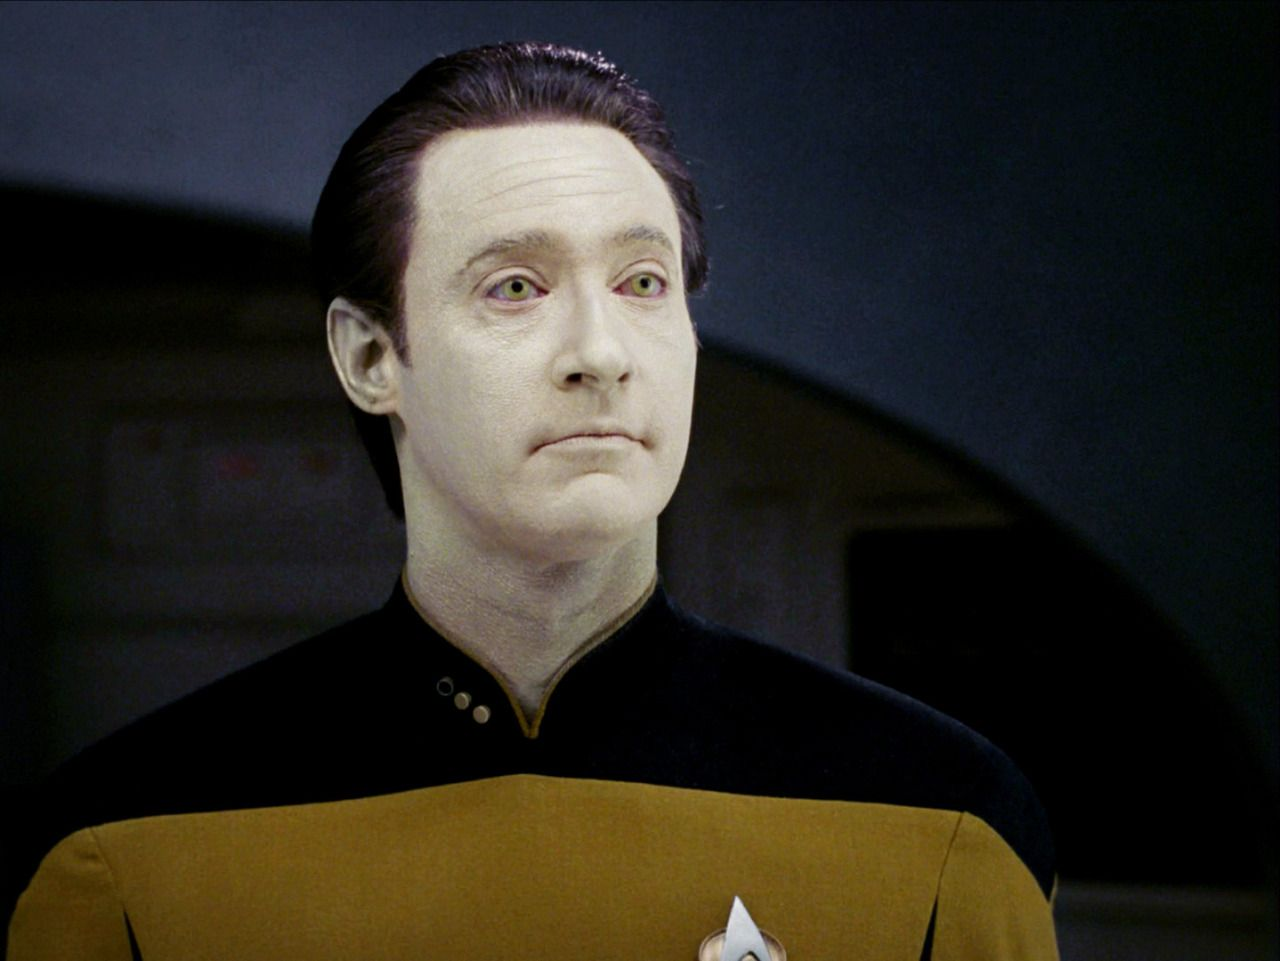
\includegraphics[width=0.4\textwidth]{images/data.jpg}
\end{center}


\end{frame}

\begin{frame}
\frametitle{To Execute a Program}

To execute a program we need:

\begin{enumerate}
	\item \textbf{Main Memory}
	\item \textbf{System Bus}
	\item \textbf{Processor}
\end{enumerate}

Of course, this is the minimal set.

\end{frame}

\begin{frame}
\frametitle{Main Memory}
Ideally, memory would be:

\begin{itemize}
	\item Fast enough that the processor never has to wait;
	\item Large enough to hold all the data;
	\item Inexpensive.
\end{itemize}

The \alert{Iron Triangle}: ``fast, good, cheap; pick two.''

Good news: we can have different levels of memory.

\end{frame}

\begin{frame}
\frametitle{Main Memory}

Let us compare the various levels I might have in my laptop from 2019:

\begin{center}
	\begin{tabular}{l|l|l}
	\textbf{Memory Level} & \textbf{Access Time} & \textbf{Total Capacity} \\ \hline
	Register & 1 ns & < 1 KB \\
	Cache & 2 ns & 16 MB \\
	Main Memory (RAM) & 10 ns & 64 GB \\
	Solid State Hard Disk & 250 $\mu$s & 1000 GB \\
	Backup Hard Disk Drive & 10 ms & 2 TB \\
	\end{tabular}
\end{center}


\end{frame}

\begin{frame}
\frametitle{Memory Access Analogy}
I am the CPU and a particular book is the piece of data needed.

If the data is in the cache: the book is on a bookshelf in my office.

If the data for the CPU on a magnetic hard disk, I have to get the book from Library and Archives Canada in Ottawa (550 km away).\\
\quad And I would have to walk.

\end{frame}

\begin{frame}
\frametitle{Memory Access Analogy}

The CPU doesn't go get the data; instead it must wait for it to arrive.

What might I do in the meantime...?

\end{frame}

\begin{frame}
\frametitle{System Bus}

This is the data transfer mechanism between most components.

It is the physical wires that connect things.

Every sort of communication using the same bus.\\
\quad Contention for this resource is a limiting factor. 

\end{frame}


\begin{frame}
\frametitle{System Buses}

The original IBM PC did work like that.\\
\quad A modern system has numerous buses.

\begin{itemize}
	\item Data Bus (memory)
	\item Address Bus (select for r/w)
	\item Instruction Bus
	\item System Bus (peripherals)
\end{itemize}

\end{frame}

\begin{frame}
\frametitle{Central Processing Unit (CPU)}

\begin{center}
	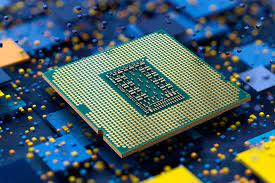
\includegraphics[width=0.4\textwidth]{images/cpu.jpg}
\end{center}


The processor (CPU) is the brain of the computer.

Fetch instructions, decode them, execute them.

Okay, there's a bit more to it than this.

\end{frame}

\begin{frame}
\frametitle{Central Processing Unit (CPU)}

Fetch-decode-execute cycle repeated until the program finishes.

Different steps may be completed in parallel (\alert{pipeline}).

Processors' largest unit is the \alert{word}.\\
\quad 32-bit computer $\rightarrow$ 32-bit word. 64-bit computer $\rightarrow$ 64-bit word.

\end{frame}

\begin{frame}
\frametitle{Central Processing Unit (CPU)}


CPU instructions are specific to the processor.

Written assembly? You might have to do some in your OS.

Some operations only available in supervisor mode.\\
\quad Attempting to run it in user mode is an error.


\end{frame}

\begin{frame}
\frametitle{Central Processing Unit (CPU)}
CPUs have storage locations: \alert{registers}.

They may store data or instructions.

Management of registers is partly the role of the OS.

Let us examine a few of the critical registers.

\end{frame}

\begin{frame}
\frametitle{CPU Registers}

A few of the registers in a typical CPU:

\begin{itemize}
	\item \textbf{Program Counter}
	\item \textbf{Status Register}
	\item \textbf{Instruction Register}
	\item \textbf{Stack Pointer}
	\item \textbf{General Purpose Registers}
\end{itemize}

\end{frame}

\begin{frame}
\frametitle{Who Manages the Registers?}

In many programs, the compiler is responsible for register assignment.

If we write an assembly program, then our responsibility!

\end{frame}

\begin{frame}
\frametitle{ARM Cortex M4 Registers}
\vspace{6em}

\begin{multicols}{2}
\begin{itemize}
	\item 13 general purpose \texttt{r0 - r12}
	\item Stack Pointer (okay, 2)
	\item Link Register
	\item Program Counter
	\item xPSR (Operating Mode)
\end{itemize}
\columnbreak

\begin{center}
  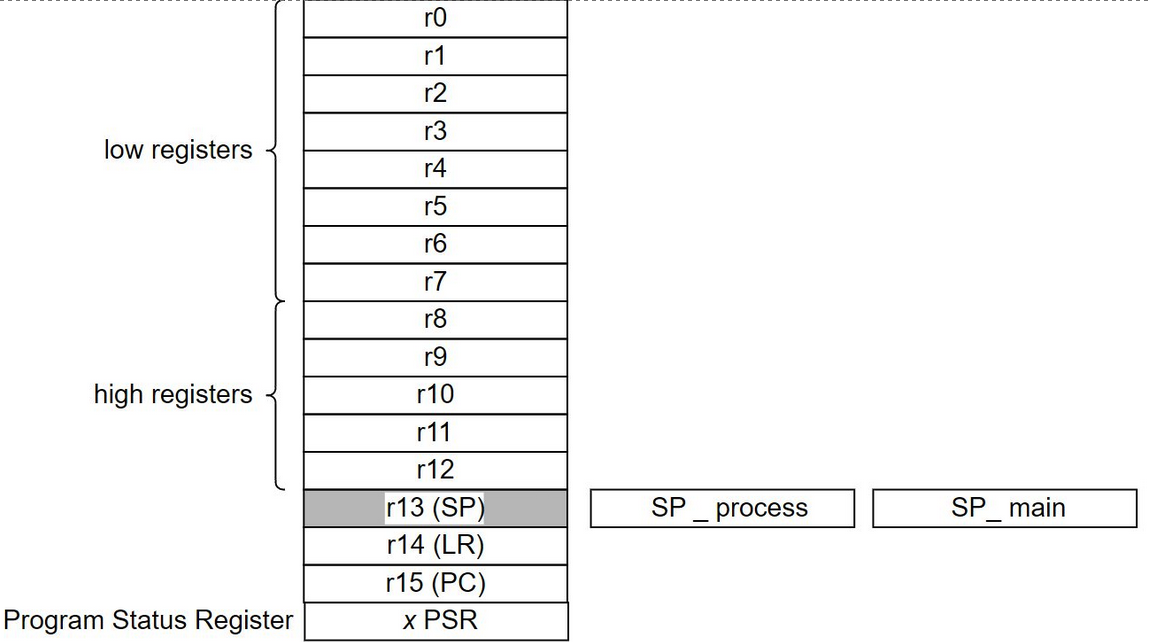
\includegraphics[width=0.5\textwidth]{images/m4registers.png}
\end{center}
\end{multicols}

\end{frame}


\begin{frame}
\frametitle{Caching}

\vspace{5em}

\begin{quote}
\textit{Caching is very... hit and miss.}
\end{quote}
\hfill - Nicholas Armstrong

\begin{center}
	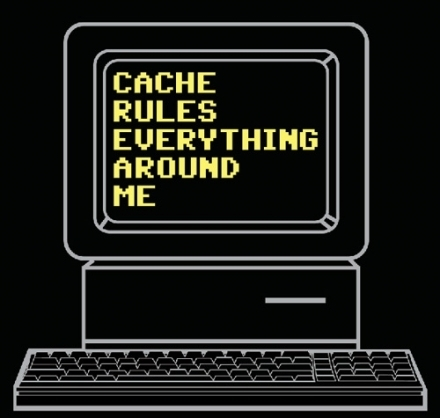
\includegraphics[width=0.4\textwidth]{images/cacherules.jpg}
\end{center}

\end{frame}

\begin{frame}
\frametitle{Caching}

Caching is very important in computing, and not just memory. 

We examine the idea of caching in the context of memory.

It is applicable any time there is a large resource that is divided into pieces, some of which are used more often than others. 

Caching provides a benefit in some circumstances; not useful in others. 


\end{frame}

\begin{frame}
\frametitle{Caching}

The goal of caching is to speed up operations. 

It is desirable to read information from cache, when possible, because it takes less time to get data from cache to the CPU than from main memory to the CPU. 

CPUs are a lot faster than memory and it is best if we do not keep them waiting.

\end{frame}

\begin{frame}
\frametitle{Doing Lines}

Caches do not have to operate on pages. 

They can operate on anything, but they are typically blocks of a given size. 

An entry in a cache is often called a \alert{line}. 

We will assume that a cache line maps nicely to a page.

\end{frame}

\begin{frame}
\frametitle{Battleship Sunk!}

As discussed, the CPU generates a memory address for a read/write operation. 

The address will be mapped to a page; ideally that page is in the cache.

\begin{center}
	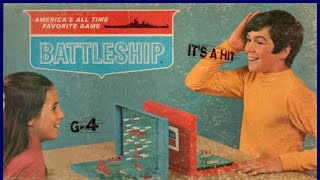
\includegraphics[width=0.5\textwidth]{images/battleship.jpg}
\end{center}

If the requested page is, in fact,  in the cache, we call that a cache \alert{hit}.

\end{frame}

\begin{frame}
\frametitle{Please Play Again}

If the page is not found in the cache, it is considered a cache \alert{miss}. 

In case of a miss, we must load the page from memory, a slow operation. 

A page miss is also called a \alert{page fault}.

\end{frame}

\begin{frame}
\frametitle{Accuracy}

The percentage of the time  a page is found in the cache is called the \alert{hit ratio}.

\begin{center}
	
\includegraphics[width=0.4\textwidth]{images/hitratio.jpg}
\end{center}

We can calculate the effective access time if we have an estimate of the hit ratio.

\end{frame}

\begin{frame}
\frametitle{Effective Access Time}

The effective access time is therefore computed as:

\begin{center}
Effective Access Time = $h \times t_{c} + (1-h) \times t_{m}$
\end{center}

Where:\\
\quad $h$ is the hit ratio.\\
\quad $t_{c}$ is the time required to load a page from cache.\\
\quad $t_{m}$ is the time to load a page from memory. 


Of course, we would like the hit ratio to be as high as possible.\\
\quad And the effective access time to be as small as possible.

\end{frame}

\begin{frame}
\frametitle{We Put a Cache in Your Cache...}

Caches have limited size, because faster caches are more expensive. 

With infinite money we might put everything in registers.

Caches for memory are very often multileveled. 

Intel 64-bit CPUs tend to have L1, L2, and L3 caches.\\
\quad L1 is the smallest and fastest;  L3 is the largest and slowest.

\end{frame}

\begin{frame}
\frametitle{Multiple Levels of Cache}

\begin{center}
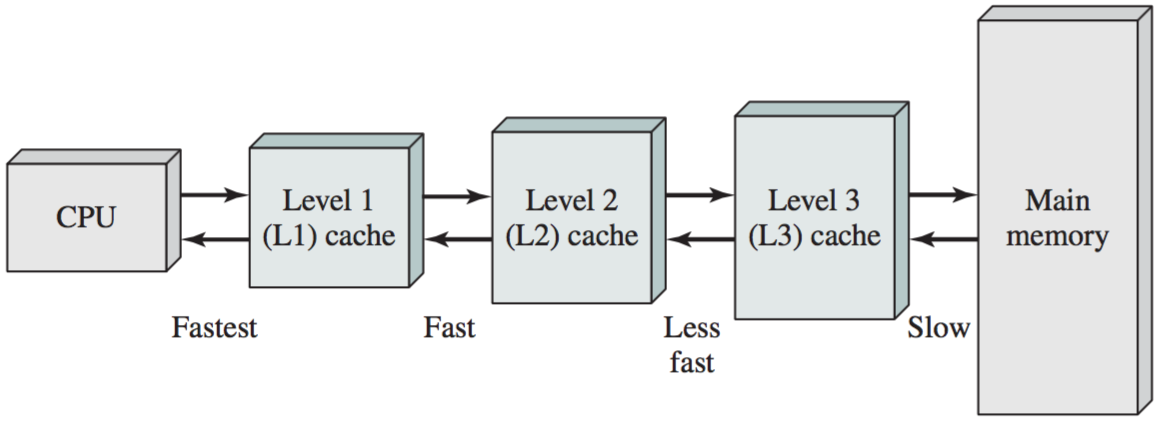
\includegraphics[width=0.9\textwidth]{images/caches.png}
\end{center}

The effective access time formula needs to be updated and expanded.

\end{frame}

\begin{frame}
\frametitle{Darn, Missed Again}

If we have a miss in the L1 cache, the L2 cache is checked. 

If the L2 cache contains the desired page, it will be copied to the L1 cache and sent to the CPU. 

If it is not in L2, then L3 is checked. 

If it is not there either, it is in main memory and will be retrieved from there and copied to the in-between levels on its way to the CPU. 

Because caches have limited size, we have to manage this storage carefully.


\end{frame}

\begin{frame}
\frametitle{Page Replacement Algorithms}

Whenever a page fault occurs, the operating system needs to choose which page to \alert{evict} from the cache to make space for the new one. 

This assumes that the cache is full, which it likely is except at system startup. 

We could, of course, just select a random page...\\
\quad We should do this task more intelligently, if we can.

\end{frame}


\begin{frame}
\frametitle{Page Replacement Algorithms}
To make an intelligent decision about what sort of strategy to choose, we need to know a few things about how data is accessed in a system.



\begin{enumerate}
	\item The 90/10 rule.
	\item The principle of \alert{temporal locality}. 
	\item The principle of \alert{spatial locality}.
\end{enumerate}

\end{frame}

\begin{frame}
\frametitle{Temporal \& Spatial Locality}

Example: a function that sums up all the values of an array. 

The sum variable is accessed repeatedly, and the fact that it was recently accessed means it is likely to be accessed again soon. 

The array being accessed at index $i$ now means it is likely that the array at index $i+1$ is likely to be accessed soon.

\end{frame}

\begin{frame}
\frametitle{Cortex M4 Flash Frames}

The Cortex M4 is a 32-bit system: instructions are (up to) 32 bits.

We can fetch more than one instruction at a time (4 to 8).\\
\quad The instruction bus is 128 bit.

Think of it like reading ahead a bit in IKEA instructions.

\end{frame}

\begin{frame}
\frametitle{Hurry Up and Wait}

The Cortex M4 requires CPU cycles be wasted to access flash.\\
\quad At 84 MHz, 6 CPU cycles wasted.

Faster CPU clock equals more waiting.

\begin{center}
  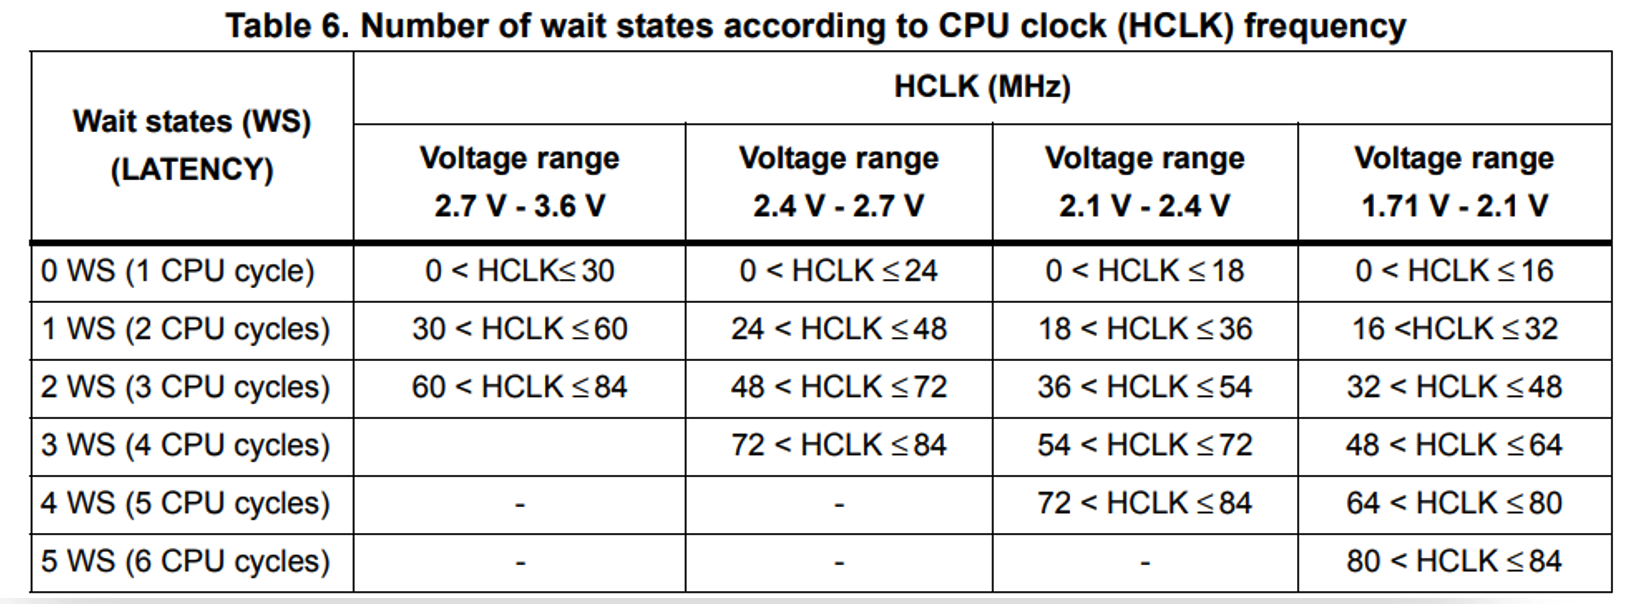
\includegraphics[width=\textwidth]{images/waitstates.png}\\
  \hfill Source: STM32 Reference Manual
\end{center}

\end{frame}

\begin{frame}
\frametitle{Sometimes We Guess Wrong}

Fetch as many instructions as we can in one go.

If we pre-fetch instructions, what if we get it wrong?

Solution in STM32F401RE: branch cache! (Be prepared)

\end{frame}

\begin{frame}
\frametitle{Goal: Reduce Waiting}

Without pre-fetch: get instructions, do them, get next instructions.

With: get instructions, do them + get next instructions in parallel.

Benefit: avoid waiting for next instructions after we're done executing.

\end{frame}

\begin{frame}
\frametitle{Split Cache: Instructions and Data}

Often instructions and data have their own caches.

Cortex M4 has a data cache of 8 $\times$ 128 bits.

\end{frame}

\begin{frame}
\frametitle{Memory Maps}

We can generate any memory address in the CPU; not everything goes to RAM.

\begin{center}
  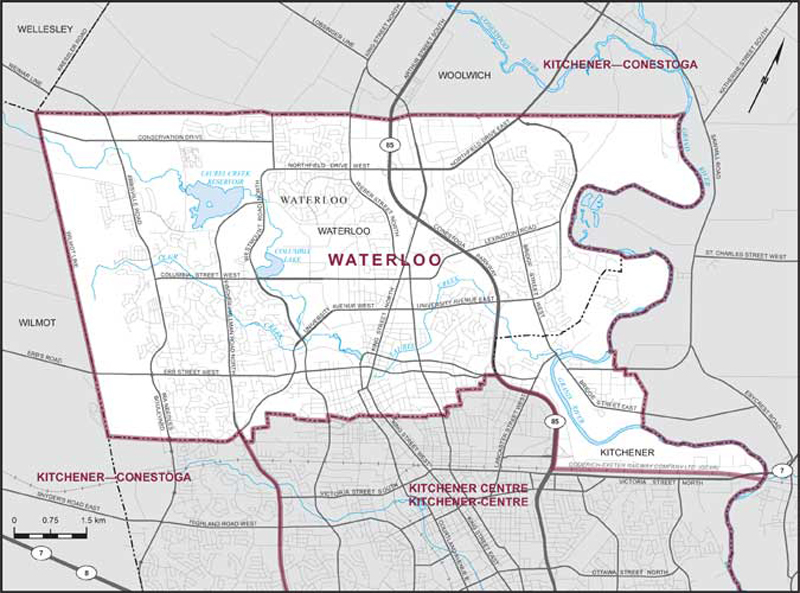
\includegraphics[width=0.6\textwidth]{images/waterloo.jpg}
\end{center}

Some addresses are reserved for I/O, peripherals, chip settings...

\end{frame}

\begin{frame}
\frametitle{Cortex M4 Memory Map Overview}

\begin{center}
  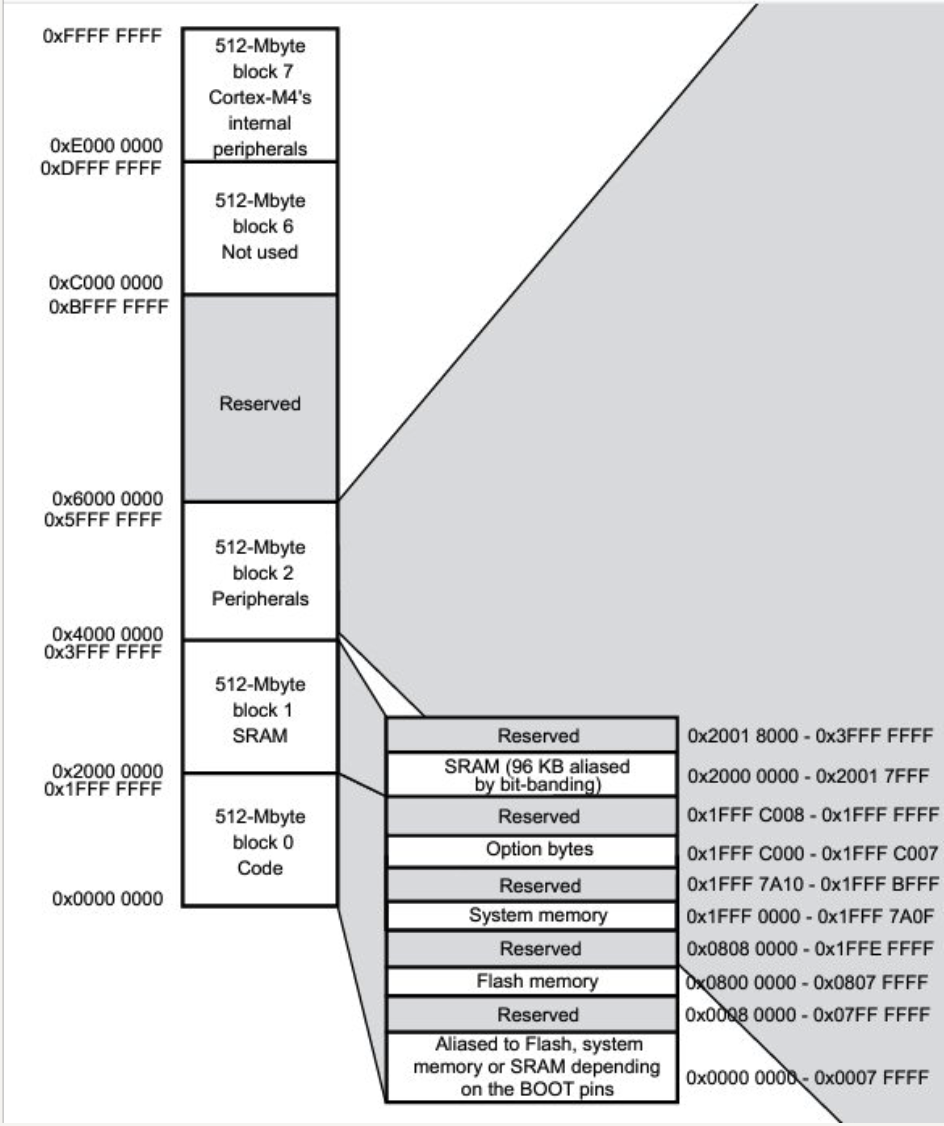
\includegraphics[width=0.5\textwidth]{images/m4memmap.png}
\end{center}

\end{frame}

\begin{frame}
\frametitle{That's Nice?}

Every kind of data (RAM, Flash, etc) are accessed via pointers.

This reduces the maximum potential size of RAM.\\
\quad Address ranges are limited.

Microcontrollers commonly do this; desktops usually do not.

\end{frame}

\begin{frame}
\frametitle{Is that it?}

\begin{center}
  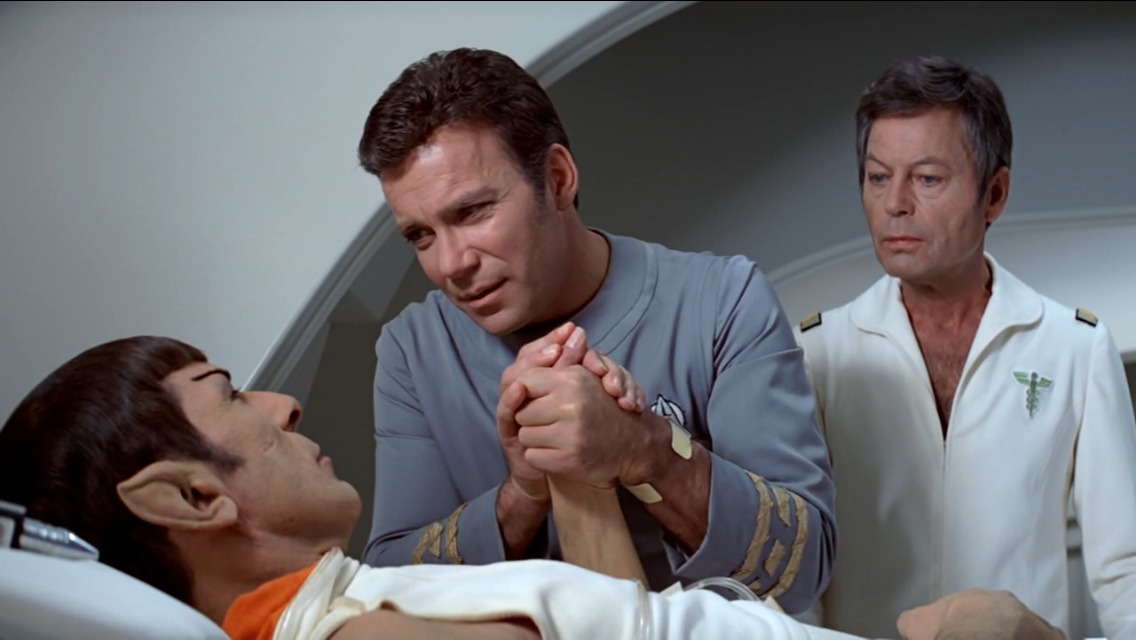
\includegraphics[width=0.4\textwidth]{images/allthatiam.png}
\end{center}\vspace{-2em}
  \textit{"Is this all that I am? Is there nothing more?"} -- Spock, sharing V'Ger's thoughts.

No! Virtual memory is \textit{much} more complicated than this.\\
\quad We'll have to revisit that subject later.

\end{frame}

\end{document}

